\documentclass[11pt]{aghdpl}
% \documentclass[en,11pt]{aghdpl}  % praca w języku angielskim

% Lista wszystkich języków stanowiących języki pozycji bibliograficznych użytych w pracy.
% (Zgodnie z zasadami tworzenia bibliografii każda pozycja powinna zostać utworzona zgodnie z zasadami języka, w którym dana publikacja została napisana.)
\usepackage[english,polish]{babel}

% Użyj polskiego łamania wyrazów (zamiast domyślnego angielskiego).
\usepackage{polski}

\usepackage[utf8]{inputenc}

% dodatkowe pakiety

\usepackage{mathtools}
\usepackage{amsfonts}
\usepackage{amsmath}
\usepackage{amsthm}
\usepackage{enumerate}
\usepackage{listings}
\usepackage{float}
\usepackage{graphicx}

% --- < bibliografia > ---
\usepackage[
style=numeric,
sorting=none,
%
% Zastosuj styl wpisu bibliograficznego właściwy językowi publikacji.
language=autobib,
autolang=other,
% Zapisuj datę dostępu do strony WWW w formacie RRRR-MM-DD.
% urldate=iso,
% Nie dodawaj numerów stron, na których występuje cytowanie.
backref=false,
% Podawaj ISBN.
isbn=true,
% Nie podawaj URL-i, o ile nie jest to konieczne.
url=false,
%
% Ustawienia związane z polskimi normami dla bibliografii.
maxbibnames=3,
% Jeżeli używamy BibTeXa:
backend=bibtex
]{biblatex}

\usepackage{csquotes}
% Ponieważ `csquotes` nie posiada polskiego stylu, można skorzystać z mocno zbliżonego stylu chorwackiego.
\DeclareQuoteAlias{croatian}{polish}

\addbibresource{bibliografia.bib}

% Nie wyświetlaj wybranych pól.
%\AtEveryBibitem{\clearfield{note}}


% ------------------------
% --- < listingi > ---

% Użyj czcionki kroju Courier.
\usepackage{courier}

\usepackage{listings}
\lstloadlanguages{TeX}

\lstset{
	literate={ą}{{\k{a}}}1
           {ć}{{\'c}}1
           {ę}{{\k{e}}}1
           {ó}{{\'o}}1
           {ń}{{\'n}}1
           {ł}{{\l{}}}1
           {ś}{{\'s}}1
           {ź}{{\'z}}1
           {ż}{{\.z}}1
           {Ą}{{\k{A}}}1
           {Ć}{{\'C}}1
           {Ę}{{\k{E}}}1
           {Ó}{{\'O}}1
           {Ń}{{\'N}}1
           {Ł}{{\L{}}}1
           {Ś}{{\'S}}1
           {Ź}{{\'Z}}1
           {Ż}{{\.Z}}1,
	basicstyle=\footnotesize\ttfamily,
}

% ------------------------

\AtBeginDocument{
	\renewcommand{\tablename}{Tabela}
	\renewcommand{\figurename}{Rys.}
}

% ------------------------
% --- < tabele > ---

\usepackage{array}
\usepackage{tabularx}
\usepackage{multirow}
\usepackage{booktabs}
\usepackage{makecell}
\usepackage[flushleft]{threeparttable}

% defines the X column to use m (\parbox[c]) instead of p (`parbox[t]`)
\newcolumntype{C}[1]{>{\hsize=#1\hsize\centering\arraybackslash}X}


%---------------------------------------------------------------------------

\author{Mateusz Grzeliński, Kornel Wilk, Mateusz Szymkowski}
\shortauthor{M. Grzeliński, K. Wilk, M. Szymkowski}

\titlePL{Uczenie populacji w oparciu o różne metody przekazywania wiedzy}
\titleEN{Collective learning}
\shorttitlePL{}
\thesistype{Modelowanie i symulacja systemów}
\degreeprogramme{Informatyka}
\date{2018}
\department{Katedra Informatyki Stosowanej}
\faculty{Wydział Elektrotechniki, Automatyki,\protect\\[-1mm] Informatyki i Inżynierii Biomedycznej}
\acknowledgements{}


\setlength{\cftsecnumwidth}{10mm}

%---------------------------------------------------------------------------
\setcounter{secnumdepth}{4}
\brokenpenalty=10000\relax

\begin{document}

\titlepages

% Ponowne zdefiniowanie stylu `plain`, aby usunąć numer strony z pierwszej strony spisu treści i poszczególnych rozdziałów.
\fancypagestyle{plain}
{
        % Usuń nagłówek i stopkę
        \fancyhf{}
        % Usuń linie.
        \renewcommand{\headrulewidth}{0pt}
        \renewcommand{\footrulewidth}{0pt}
}

\setcounter{tocdepth}{2}
\tableofcontents
\clearpage

\chapter{Wstęp}
\section{Opis problemu}

\section{Pojęcia, przykłady, zjawiska}
\begin{enumerate}
\item Barwy organizacji \cite{ReinventingOrganizations} -- rózne sposoby zarządznia ukazanie za pomocą różnych barw, gdzie turkusowy odpowiada samozarządzanu, a czerwony silnemu autorytytowi przywódcy
\item Eksperyment setnej małpy \cite{EksperymentSetnejMalpy} -- wiedza zdobyta przez jednostkę przechodzi na cały gatunek, należy traktować jako przykład, nie twierdzenie
\item Eksperyment więzienny \cite{EksperymentWiezienny} -- jak zachowuje się człowiek, jeśli ma władzę nad drugim, również odwrotnie, należy traktować jako przykład, nie twierdzenie


\end{enumerate}

\section{Artykuły naukowe}
\begin{enumerate}

\item Multi-agent systems and role games: collective learning processes for ecosystem management\cite{MultiAgentSystemsAndRoleGamesCollectiveLearningProcessesForEcosystemManagement}

Systemy wieloagentowe świetnie nadają się do symulacji dynamicznie zmieniającego się zbioru graczy chcących osiągnąć swoje rezultaty. Ponadto ich ciekawym i użytecznym zastosowaniem jest zamodelowanie wystąpienia ograniczonego zasobu i jego eksploatacji przez różnych graczy. Same role-games są tworem o podobnym skomplikowaniu co systemy wieloagentowe, a co za tym idzie systemy wieloagentowe mogą zostać wdrożone do symulacji takich gier, a sama gra może dostarczyć interesujących modeli zachowań, które następnie mogą zostać użyte do symulacji za pomocą systemu wieloagentowego.
Także chcąc zdobyć przykłady do zamodelowania systemu wieloagentowego symulującego dane zagadnienie moożna skonstruować grę która służyć będzie do badania zachowania graczy-agentów w różnych sytuacjach i pomoże dostosować parametry agentów teprezentujących różne podejścia.


\item Impact of social media on collective learning \cite{ImpactOfSocialMediaOnCollectiveLearning}

Collective learning jest zarówno konwersacją bezpośrednią jak i na odległość. Wcześniejsza w rozwoju wersja to collectiva learning na spotkaniach służących wymianie wiedzy. Chęć skorzystania z danego sposobu nauki zależy od tego jak wygodnie się z niego korzysta i na ile uważa się, że poszerza on wiedzę uczącego się. Social media pozytywnie wpływają na chęć nauki i rezultaty uzyskiwane w jej trakcie.

\item Conceptualizing Collective Learning and Knowledge Building in the context of migration and development \cite{ConceptualizingCollectiveLearning}

Typy wiedzy:

\begin{itemize}
        \item Wiedza zdobyta przez doświadczenie, rozumienie danej rzeczy
        \item Świadomość istnienia czegoś
        \item Wiedza jako wyprowadzona przez rozumowanie
        \item Posiadanie informacji lub zostanie nauczonym
\end{itemize}

Można podzielić też ze względu na sposób przechowywania:

\begin{itemize}
        \item Wewnętrzna- zdobyta przez doświadczenie lub wymianę wiedzy, polega na między innymi na rozumieniu danego zjawiska, nie da się jej ująć językiem czy formułami matematycznymi
        \item Zewnętrzna- zapisana w jakiś sposób na zewnętrznym nośniku, nie jest przechowywana w umyśle, lecz np.: w książce, malowidłach itp. Jest ona bardziej uniwersalna, gdyż jej celem jest bycie zrozumiałą dla szerokiego kręgu odbiorców, wyrażona językiem, bądź regułami
\end{itemize}

Mądrość jest znajomością powodów, reguł, schematów które można wyprowadzić z danych, ale które również mogą służyć do przewidywania rzeczywistości.

Nauka może być przeprowadzona przez:
\begin{itemize}
        \item Rozumowanie i dzielenie wiedzy
        \item Działanie
\end{itemize}

Collectiva learning ma na celu podzielenie się wiedzą przez uczestników, wymianę wiedzy, danych, refleksja nad nimi i efekt/odpowiedź

\item Waves: a model of collective learning \cite{WavesModelOfCollectiveLearning}

Dla urealnienia sytuacji należy założyć, że nie każdy agent ma połączenie z każdym, lecz są oni częścią sieci reprezentującej kontakty i powiązania.
Przykładowy model to:

\begin{itemize}
        \item N agentów w sieci G
        \item Agenci mają jeden cel, jest nim budowa modelu z obserwacji
        \item Istnieje model który nie będzie sprzeczny z jakąkolwiek informacją uzyskaną przez obserwacje
        \item Każdy agent umie się uczyć to znaczy zaktualizować model, by nie był sprzeczny z obserwacjami o których wie
        \item Interakcja między agentami polega na zapytaniach gdzie a1 proponuje a2 pewien model a - następnie czeka na kontrargumenty ze strony a2, które przeczą temu modelowi
        \item Agenci dają poprawne odpowiedzi na zapytania
        \item W dowolnym momencie agent może dostać nowe informacje
        \item W każdym momencie jest zbiór niezależnych, równoczesnych komunikacji
\end{itemize}

Nauka kończy się gdy każdy agent ma model spójny z całością obserwacji

Każde z powyższych sztywnych założeń można zrelaksować, na przykład proces interakcji przestawić jako proces argumentacji gdzie do obalenia argumentu trzeba odpowiednich kontrargumentów. Tak samo oprócz dzielenia się argumentami mogą też dzielić się hipotezami.
By zapewnić spójną propagację informacji można dodać agentom następujące zachowanie : Za każdym razem, gdy agent zaadaptuje hipotezę innego agenta to w interakcji ze swoimi sąsiadami traktuje ją jako swoją własną. Ale w takiej sytuacji nie da się wykonać wszystkich operacji na raz.

Można również zaimplementować etapowe dzielenie wiedzy. Wtedy agenci wracają z wiedzą, dzielą się nią aż do osiągnięcia spójności, a następnie rozpoczyna się następna tura. Oczywiście wymiana wiedzy i osiągnięcie spójnego zbioru hipotez nie odbywa się bez kosztu, więc w zależności od topologii i kosztu wymiany wiedzy może się okazać, że zbyt duży koszt spowoduje zmniejszenie skuteczności przez mniejszą możliwość pozyskiwania obserwacji.

Poszczególne hipotezy można przyrównać, czy są spójne z danym zbiorem obserwacji, co znaczy, że :
\begin{itemize}
        \item Nie ma w niej żadnej obserwacji negatywnej np. dla rozmieszczenia zasobu mogłaby to być obserwacja, że na danym miejscu zasobu nie ma
        \item W hipotezie uwzględnione są wszystkie obserwacje pozytywne
\end{itemize}

Działanie poszczególnych populacji można podzielić na etapy :

\begin{itemize}
        \item Zbieranie wiedzy – agenci zbierają wiedzę
        \item Faza nauki – agenci uczą się i dochodzą do zbioru spójnych hipotez
\end{itemize}

\item Learning-by-doing \cite{LearningByDoing}

Ten artykuł pokazuje w jaki sposób opisać modelem matematycznym zjawisko uczenia jednostki jak również społecznośći. Przy założeniach:

\begin{itemize}
        \item nauka (zdobywanie doświadczenia) jest równoważna pracy
        \item jednostka posiada pewną początkową wiedzę
        \item doświadczenie to ilośc wykonanej dotychczas pracy
\end{itemize}

Zauważono następujące cechy/wnioski:

\begin{itemize}
        \item krzywa uczenia jednostki jest w przybliżeniu funkcją ekspotencjalną
        \item agent może uczyć się od każdego innego agenta, zdoność uczenia agenta X od agenta Y jest definiowana przez macierz współczynników
        \item rozwiązanie zagadnienia optymalnego uczenia nie zależy od początkowych umiejętności agenta, gdzie zagadnienie optymalnego uczenia to maksymalizacja wyniku przy zadanym czasie i objętości pracy
\end{itemize}

\item Bee colony optimization – a cooperative learning approach to complex transportation problems \cite{BeeColonyOptimization}

Proces Collective Learning można w ciekawy sposób zaprezentować za pomocą zachowania pszczół w ulu, a dokładnie na podstawie ich metod zdobywania nektaru.Odbywa się to na założeniu, że każda podąża do źródła nektaru  za pszczołą, która dotarła już do skupiska kwiatów.  Każdy ul posiada tak zwany “parkiet do tańczenia”, na którym każda pszczoła, która odkryła nowe źródło może “tańczyć” by przekonać pozostałe pszczoły do tego, by za nią podążały. Jeśli jakakolwiek pszczoła postanowi wylecieć z ula w celu zdobycia pokarmu, zrobi to za pszczołą, która wcześniej “tańczyła”. Po powrocie do ula z zebranym nektarem, pszczoła ma 3 możliwości postępowania:
\begin{itemize}
        \item porzucić źródło pokarmu i zostać od nowa “pszczołą niezależną”
        \item kontynuować zbieranie pokarmu bez “rekrutowania”
        \item “tańczyć” przed wylotem do źródła pokarmu i dzięki temu rekrutować nowe pszczoły
\end{itemize}

Każda z pszczół, która rekrutuje inne pszczoły na konkretny obszar “tańczy” w inny sposób.
Mechanizm, na podstawie którego pszczoły wybierają, za którą pszczołą podążać nie jest do końca opisany, ale można twierdzić, że jest on powiązany z jakością pokarmu, który jest uzyskiwany z danego obszaru. Warto zauważyć, że nie wszystkie pszczoły wyruszają by zdobyć nektar w tym samym momencie, więc ich działanie nie jest synchronizowane. Zostało jednak udowodnione, że liczba nowych pszczół, które będą wylatywały by zbierać nektar jest proporcjonalna do różnicy ilości wszystkich pszczół i tych obecnie zbierających.

Na podstawie obserwacji zachowania pszczół można napisać algorytm, który będzie w pewien sposób symulował ich zachowanie:

Bee Colony Optimization
\begin{enumerate}
        \item[$1)$] Initialization. Determine the number of bees B, and the number of iterations I. Select the set of stages ST = {st1, st2 ,…, stm}. Find any feasible solution x of the problem. This solution is the initial best solution.
        \item[$2)$] Set i: = 1. Until i = I, repeat the following steps:
        \item[$3)$] Set j = 1. Until j = m, repeat the following steps:
                Forward pass: Allow bees to fly from the hive and to choose B partial solutions from the set of partial solutions Sj at stage stj .
                Backward pass: Send all bees back to the hive.
                Allow bees to exchange information about quality of the partial solutions created and to decide whether to abandon the created partial solution and become again uncommitted follower, continue to expand the same partial solution without recruiting the nestmates, or dance and thus recruit the nestmates before returning to the created partial solution. Set, j: = j + 1.
        \item[$4)$] If the best solution xi obtained during the i-th iteration is better than the best- known solution, update the best known solution (x: = xi).
        \item[$5)$] Set, i: = i + 1
\end{enumerate}

Inny model, który został stworzony to taki, że każda pszczoła posiada następujące cechy:
\begin{itemize}
\item physical properties:
        \begin{itemize}
                \item position (x, y)
                \item position (x, y) 50 m/min)
                \item position (x, y)
        \end{itemize}
\item perceptual properties:
        \begin{itemize}
                \item visual Distance outside (max.: 25 m)
                \item hear Distance inside (max.: 0.1 m)
                \item (smell Distance)
        \end{itemize}

\item memorizing properties:

        \begin{itemize}
                \item time Of Day Found
                \item position (distance from hive; direction from hive)
                \item profitability( =concentration)
                \item (odour)
                \item (colour)
        \end{itemize}

        \begin{itemize}
                \item motivational properties (states):
                \item homing Motivation (varies between 0 and 1)
                \item foraging Motivation (0 or 1)
                \item abandoning Tendency (varies between 0 and 1)
        \end{itemize}
\end{itemize}

Ogólne zasady, każda pszczoła może lecieć maksymalnie na 500m odległość od ula, po przekroczeniu tej granicy od razu wraca do ula. By przekazać wiedzę, gdzie znajduje się lokalizacja miejsca z którego pobierane są zasoby, każda pszczoła musi wykonywać “taniec”.  Został stworzony parametr “transmission accurancy”, który definiuje “writting error” i “transmission error”, podczas wykonywania “tańca” jak i jego “odczytywania”.


\end{enumerate}

\section{Opis modelu}

Model przedstawia zdobywanie i rozprzestrzenianie się wiedzy w społeczeństwie. Pierwszym z założeń modelu jest skwantyfikowanie czasu, który jest reprezentowany przez poszczególne tury. Dla odwzorowania procesu założyliśmy, że społeczeństwo zostanie zaprezentowane jako sieć znajomości, przestawiona na grafie nieskierowanym. Graf ów przedstawia możliwe ścieżki przekazywania wiedzy między poszczególnymi osobnikami w populacji (dalej zwanymi agentami) i stanowi element odpowiadający za symulację społeczeństwa zdolnego do wymiany wiedzy. Za pomocą sieci połączeń można zamodelować zarówno strukturę społeczeństwa, jak i różne sposoby dzielenia się wiedzą. Drugim istotnym czynnikiem który braliśmy pod uwagę była niedoskonałość przekazywania wiedzy, którą reprezentuje współczynnik szansy przekazania wiedzy, który określa średnie zdolności poznawczo-kognitywne agentów należących do danego społeczeństwa. Każdy agent posiadać może wiedzę o zasobie, która dla zasymulowania działania jej przekazywania jest charakteryzowania przez jej wiek. Wiek wiedzy determinuje jak daleko może się ona rozprzestrzenić od agenta ją rozpowszechniającego. Ponadto agent posiada przypisanie czyli wiedzę o pojedynczym zasobie który został mu przypisany i do którego ma dostęp na wyłączność. Środowisko jest zamodelowane za pomocą dwu wymiarowej mapy z polami na których może się znajdować pewna ilość zasobu. Agenci nie mający przypisanego zasobu zbierają wiedzę sprawdzając w każdej turze losowe pole, jeżeli znajdzie wiedzę to oznacza to pole jako znalezione (ustawia 0 w ilości zasobu, do swojej wiedzy zapisuje il. Zasobu z pola -1, a sobie przypisuje zasób). Następnie odbywa się wymiana wiedzy. Agenci mający wiedzę przeszukują swoje sąsiedztwo w odległości równej wiekowi ich wiedzy, a poruszając się tylko po węzłach grafu na których agenci już mają przypisanie. Jeżeli w takim sąsiedztwie natrafią na agenta nieposiadającego wiedzy to przekazuję mu ją (nadają przypisanie) i zmniejszają w swej wiedzy ilość zasobów, gdyż przypisany został już jeden z nich innemu agentowi.

Podsumowując Agenci współpracują ze sobą i nie podbierają sobie zasobów, jeżeli agent ma przypisany zasób to nie szuka kolejnych, tylko eksploatuje nadany, a agenci z wiedzą rozprzestrzeniają ją arbitralnie do swych sąsiadów mając na celu powiększenie ilości agentów z wiedzą, a gdy przekażą ją ilości agentów równej ilości zasobów jaką znaleźli, to przestają rozpropagowywać swoją wiedzę i jedynie zbierają zasób i uczestniczę w przeazywaniu wiedzy po sieci powiązań.

\section{Opis techniczny}

Do realizacji naszego projektu skorzystaliśmy z języka programowania pyton, w szczególności z biblioteki networkx do tworzenia i obsługi grafów, numpy, do reprezentacji wiedzy, oraz matplotlib.pyplot do tworzenia wykresów danych wynikowych.
Program można uruchomić za pomocą $main.py –h$
Możliwości programu:

\begin{itemize}

\item  max\_iterations - określa maksymalną ilość iteracji którą program wykona, gdzie iteracja jest turą zbierania i dzielenia się wiedzą.
\item  map\_size – określa długość boku kwadratowej mapy zasobów
\item  number\_of\_cells\_with\_resources – oznacza ilość pól na których będą zasoby
\item  value\_of\_resource – oznacza ile zasobów będzie na każdym z wylosowanych pól
\item  number\_of\_cliques – oznacza ilość klik w caveman\_connected\_graph
\item  clique\_size – oznacza wielkość klik (grup agentów które składają się z jednakowej liczby agentów połączonych grafem pełnym)
\item p – parametr oznaczający procentową szansę na przekazanie wiedzy

\end{itemize}

Program składa się z trzech głównych funkcji:

\begin{itemize}

\item Get\_knowledge – odpowiada za znajdowanie wiedzy przez agentów,
\item Share\_knowledge – odpowiada za przekazywanie sobie wiedzy przez agentów.
\item Iterate\_knowledge – odpowiada za czas, przebieg poszczególnych etapów rozwoju wiedzy w populacji, a także za zapisywanie wyników.

\end{itemize}

\section{Statystyki}

Przykładowe wykresy przedstawiające ilość zdobytej wiedzy wraz z upływem czasu (iteracji).
\nopagebreak

\begin{figure}[H]
	\centering
	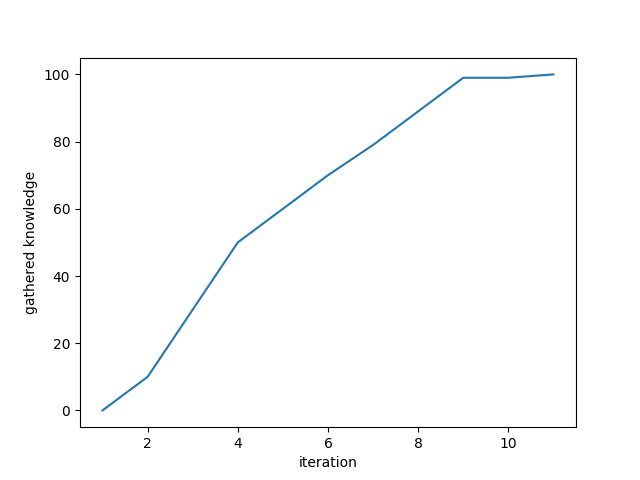
\includegraphics[width=130mm]{wykresy/learning_map-50x50_graph-2-50_res-10-100_p-1.png}
	\caption{Wykres dla mapy 20x20, 2 kliki, 100 agentów, 10 zasobów o wartości 100}
\end{figure}

\begin{figure}[H]
	\centering
	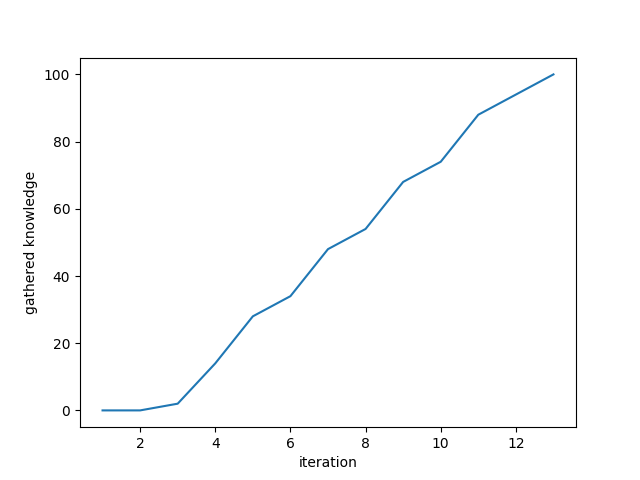
\includegraphics[width=130mm]{wykresy/learning_map-50x50_graph-20-5_res-10-100_p-1.png}
	\caption{Wykres dla mapy 20x20, 20 klikek, 100 agentów, 10 zasobów o wartości 100}
\end{figure}

Poniższe wykresy przedstawiają szybkość zdobywania wiedzy przez populację (ilośc iteracji potrzebnej do zebrania całej dostępnej wiedzy) w zależnośći ilości klik.
\nopagebreak

\begin{figure}[H]
	\centering
	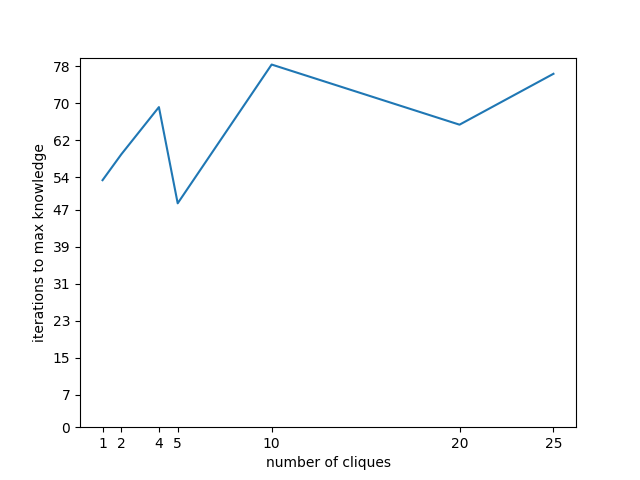
\includegraphics[width=130mm]{wykresy/different_number_of_cliques_map-20x20_graph-10-10_res-10-10_p-1.png}
	\caption{Wykres dla mapy 20x20, 100 agentów, 10 zasobów o wartości 10}
\end{figure}

Poniższe wykresy przedstawiają szybkość zdobywania wiedzy przez populację (ilośc iteracji potrzebnej do zebrania całej dostępnej wiedzy) w zależnośći od zasobów dostępnych na mapie.
\nopagebreak

\begin{figure}[H]
	\centering
	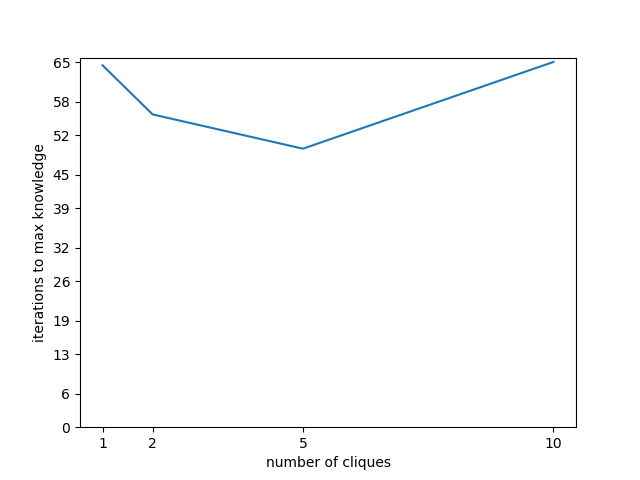
\includegraphics[width=130mm]{wykresy/different_number_of_cliques_map-20x20_graph-1-100_res-10-10_p-1.png}
	\caption{Wykres dla mapy 20x20, 1 kliki, 100 agentów, 10 zasobów o wartości 10}
\end{figure}

\begin{figure}[H]
	\centering
	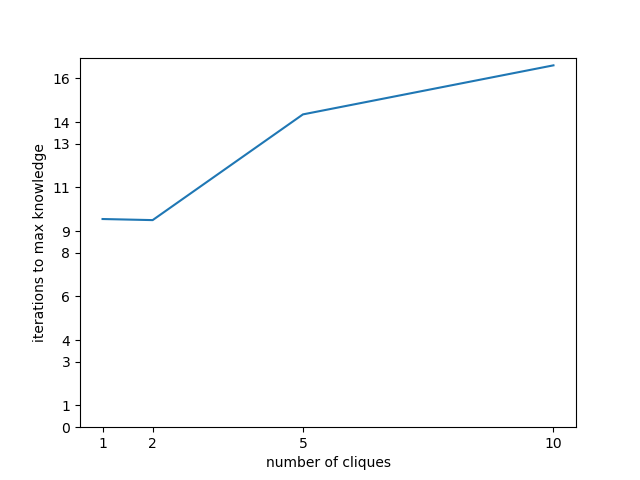
\includegraphics[width=130mm]{wykresy/different_number_of_cliques_map-20x20_graph-1-100_res-2-50_p-1.png}
	\caption{Wykres dla mapy 20x20, 1 kliki, 100 agentów, 2 zasobów o wartości 50}
\end{figure}

\begin{figure}[H]
	\centering
	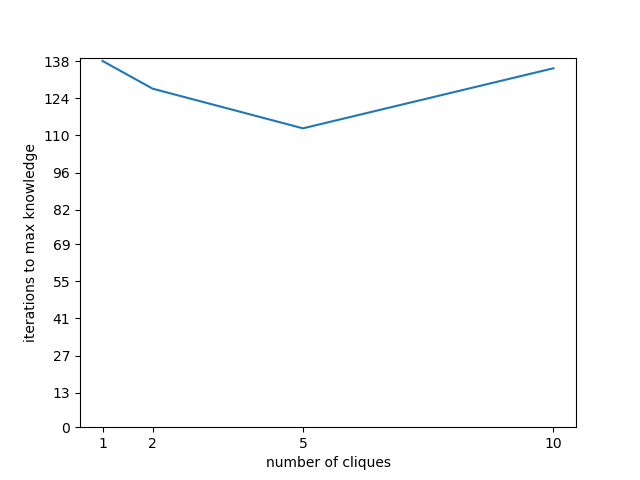
\includegraphics[width=130mm]{wykresy/different_number_of_cliques_map-20x20_graph-1-100_res-20-5_p-1.png}
	\caption{Wykres dla mapy 20x20, 1 kliki, 100 agentów, 20 zasobów o wartości 5}
\end{figure}

\begin{figure}[H]
	\centering
	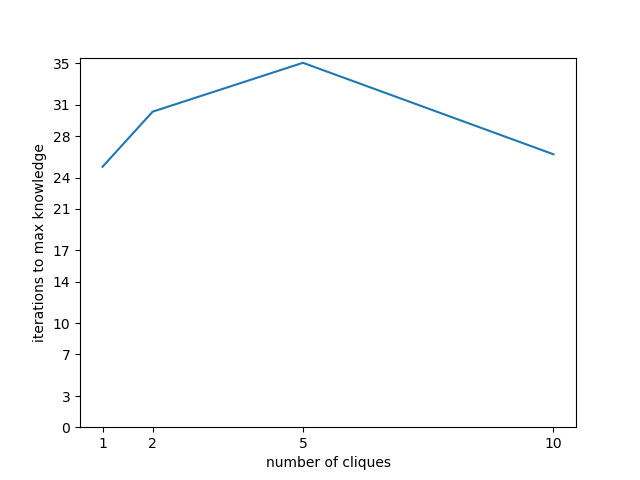
\includegraphics[width=130mm]{wykresy/different_number_of_cliques_map-20x20_graph-1-100_res-5-20_p-1.png}
	\caption{Wykres dla mapy 20x20, 1 kliki, 100 agentów, 5 zasobów o wartości 20}
\end{figure}

Wykres przedstawia zależność szybkości zdobywanej wiedzy od parametry p - prawdopodobieństwa przekazania wiedzy.
\nopagebreak

\begin{figure}[H]
	\centering
	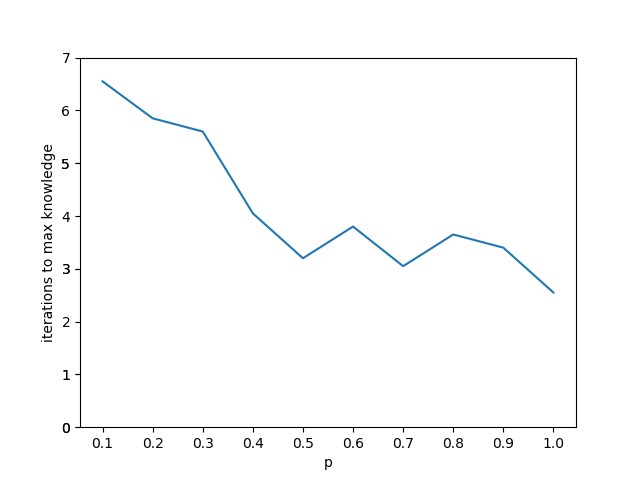
\includegraphics[width=130mm]{wykresy/different_p_map-30x30_graph-1-125_res-50-23_p-1.png}
	\caption{Wykres dla mapy 30x30, 1 kliki, 125 agentów, 50 zasobów o wartości 23}
\end{figure}


\section{Wnioski}

Zwiększanie parametru p-prawdopodobieñstwa przekazania wiedzy zwiększa szybkość zdobycia wiedzy przez całą populacje niezalełnie od ilości klik jak i ilości agentów w danej klice.

Zwiększanie ilości klik wpływa na zmniejszenie szybkości rozchodzenia się więdzy w populacji. Mniejsza ilość połączeń w grafie, powoduje mniejsze rzeczywiste prawdopodobieństwo przekazania wiedzy efekt warunkowania zdarzeñ. Występują jednak anomalnie takie jak na (zał.1). W specyficznych sytuacjach gdy ilość zasobów dostępnych przewyższa ilość dostępnych aktorów, populacja dąży do eksploatacji jednego źródła, zamiast synchronicznego pobierania z większej ilości źródeł. Problem ten zostaje rozwiązany dzięki większej ilości klik, gdyż mniejsze szansa na rozprzestrzenienie się wiedzy wewnątrz populacji zmusza innych aktorów do poszukiwania zamiast eksploatacji.


Prędkość zdobywania wiedzy jest wprost skorelowana z ilością zasobu dostępnego z konkretnego pola. Jeśli ilość aktorów w klice jest równa iloćci dostępnego zasobu z danej kliki cała klika skupia się na eksploatacji danego źródła przez co zmniejsza ona ogólne prawdopodobieñstwo uzyskania wiedzy przez pozostałą część populacji. Jeśli natomiast ilość dostępnego zasobu z konkretnego źródła przewyższa ilość aktorów w klice, to wiedza zostanie dalej przekazana do pozostałych klik, nie zmuszając ich do ponowego odkrywania danego źródła. W przeciwnej sytuacji, jeśli ilość dostępnego zasobu jest zdecydowanie mniejsza od ilości aktorów w klice pewna część danej kliki, która nie eksploatuje tego źródła, będzie miała mniejszą szansę na zdobycie wiedzy, co wydłuży czas pozyskiwania wiedzy przez całą populację.


\printbibliography

\end{document}
